\chapter{Analyse / Fit} \label{kap:analyse}
Um aus einem Datensatz den \glqq wahren\grqq\ Wert diverser Parameter abzuschätzen, gibt es verschiedene Möglichkeiten. In dieser Analyse wird die Methode sFit verwendet. Diese stellt eine modifizierte Variante des \glqq Unbinned Maximum Likelihood\grqq\ Fits dar. Unbinned meint, dass das Fitergebnis nicht von der Wahl der Säulen (engl. bins) eines Histogramms abhängt. Die Modifikation des Fits besteht in der Verwendung der aus der \SPlot-Technik bekannten sWeights. Dadurch ist es nicht nötig, den Untergrund zu modellieren, da dieser aus statistischen Gründen annihiliert wird.

\section{Maximum Likelihood Funktion}
Die Maximum Likelihood Methode ist eine weit verbreitete Methode, um Parameter abzuschätzen. Für eine gegebene Wahrscheinlichkeitsdichtefunktion (WDF) $\mathcal{P}(\vec{x_e};\vec{\lambda})$ mit einem unbekannten Satz Parametern $\vec{\lambda}$ und $N$ unabhängigen Messungen $\vec{x_e}$ ist die Likelihood-Funktion als
\begin{align}
\mathcal{L}(\vec{\lambda}) = \prod_{e=1}^N \mathcal{P}(\vec{x_e};\vec{\lambda})
\end{align}
definiert. Der Satz an Parametern, der $\mathcal{L}$ maximiert, gilt als beste Abschätzung von $\vec{\lambda}$. In der Praxis jedoch minimiert man äquivalent $-\ln\mathcal{L}$. Gewöhnlicherweise berücksichtigt man möglichen Untergrund, indem man die WDF in einen Signal- und Untergrundanteil aufteilt:
\begin{align}
\mathcal{P}(\vec{x_e};\vec{\lambda}) = f_{sig}\mathcal{P}_{sig}(\vec{x_e};\vec{\lambda}) + (1-f_{sig})\mathcal{P}_{bkg}(\vec{x_e}). \label{eq:likelihood_sig_bkg}
\end{align}
$f_{sig}$ bezeichnet hierbei den Signalanteil, $\mathcal{P}_{sig}, \mathcal{P}_{bkg}$ die WDF des Signals bzw. Untergunds. Die Schwierigkeit besteht nun darin, den Untergrund geeignet zu modellieren. Dazu bedarf es MonteCarlo-Studien oder der Verwendung separater Seitenbänder. \cite{sfit}

\section{Fitmethode sFit} \label{kap:sfit}
Der sFit bietet nun eine Möglichkeit, ohne genaue Kenntnis des Hintergrunds die wahre Verteilung des Signalanteils von $\vec{x}$ zu rekonstruieren. Dazu bedarf es einer weiteren Variable $\vec{y}$, die vollkommen unkorreliert ist, also sowohl für Signal als auch Untergrund. In dieser Analyse wird später $\vec{y} = y = M($\Bd$)$ die rekonstruierte Masse der \Bd\ sein, $\vec{x}^T = (t,d,\eta)^T$, die Variablen, die zur Bestimmung von $\SJPsi$ notwendig sind. Was diese im Einzelnen bedeuten, wird später behandelt.

Sei $N_s$ die Zahl an Signal- und $N_b$ die Zahl an Untergrund-Ereignissen eines Datensatzes. Die Verteilungen von Signal und Untergund seien mit $F_s(y)$ bzw. $F_b(y)$ bezeichnet und all diese vier Größen seien bekannt. Dann stellt die \SPlot-Technik (\cite{splot}) mit den sogenannten \glqq sWeights\grqq 
\begin{align}
W_s(y) = \frac{V_{ss}F_s(y)+V_{sb}F_b(y)}{N_sF_s(y)+N_bF_b(y)}
\end{align} 
einen Formalismus zur Verfügung, um durch Gewichtung der Ereignisse Signal vom Untergrund zu bereinigen. Die Matrix $V_{ij}$ bezeichnet dabei das Inverse der Kovarianzmatrix
\begin{align}
V_{ij}^{-1} = \sum_{e=1}^N \frac{F_i(y_e)F_j(y_e)}{(N_sF_s(y_e)+N_bF_b(y_e))^2}.
\end{align}
In der \SPlot-Technik werden die Gewichte $W_s(y_e)$ berechnet und anschließend ein Histogramm mit den Messungen $x_e$ mit der entsprechenden Gewichtung gefüllt, um die wahre Verteilung von x zu erhalten. Beim sFit wird nun die Likelihood Funktion gemäß
\begin{align}
\mathcal{L}_W(\vec{\lambda}) = \prod_{e=1}^N \mathcal{P}(\vec{x_e};\vec{\lambda})^{W_s(y_e)}
\end{align}
gewichtet. Die Erwartung ist, dass der Untergrundanteil auf statistischer Grundlage eliminiert wird und der wahre Wert von $\vec{\lambda}$ durch Maximierung von $\mathcal{L}_W(\vec{\lambda})$ abgeschätzt werden kann. \cite{sfit}

\section{Fit der Massenverteilung und Bestimmung der sWeigths} \label{kap:massenfit}
Wie bereits in Kapitel \ref{kap:sfit} erwähnt, wird die rekonstruierte Masse zur Berechnung der sWeights herangezogen. Dazu wird ein klassischer Maximum Likelihood Fit durchgeführt, d.h. Signal und Untergrund werden gemäß Gleichung \ref{eq:likelihood_sig_bkg} gesondert beschrieben.

Für den Signalteil der Massenverteilung wird ein doppelter Gauß der Form
\begin{align}
\mathcal{P}_{m;S}(m;\vec{\lambda}_{m;S}) = f_{S,m}\mathcal{G}(m;m_{\text{\Bd}},\sigma_{m,1}) + (1-f_{S,m})\mathcal{G}(m;m_{\text{\Bd}},\sigma_{m,2})
\end{align}
mit gemeinsamen Mittelwert $m_{\text{\Bd}}$, unterschiedlichen Breiten $\sigma_{m,1}$ und $\sigma_{m,2}$ sowie dem relativen Beitrag $f_{S,m}$ der beiden Gauß-Kurven angenommen. Die Normierung ist dabei bereits in $\mathcal{G}$ enthalten.

Der Untergrund wird durch die Exponentialfunktion
\begin{align}
\mathcal{P}_{m;B}(m;\vec{\lambda}_{m;B}) = \frac{1}{\mathcal{N}_{m;B}}\e^{-\alpha_m m}
\end{align}
modelliert. $\mathcal{N}_{m;B}$ bezeichnet dabei die Normierung auf den im Fit verwendeten Massenbereich $m \in [5230,5330]\mega\electronvolt/c^2$. Damit lautet die gesamte Wahrscheinlichkeitsdichtefunktion der Massenverteilung
\begin{align}
\mathcal{P}_{m}(m;\vec{\lambda}_{m}) = f_{sig}\mathcal{P}_{m;S}(m;\vec{\lambda}_{m;S}) + (1-f_{sig})\mathcal{P}_{m;B}(m;\vec{\lambda}_{m;B}) \label{eq:pdf_masse},
\end{align}
wobei $f_{sig}$ den Anteil des Signals angibt.

Der Fit liefert für den Parametersatz $\vec{\lambda}_{m}^T = (f_{sig}, f_{S,m}, m_{\text{\Bd}}, \sigma_{m,1},\sigma_{m,2}, \alpha_m)^T$ die in Tabelle \ref{tab:fit_masse} aufgeführten Resultate. Alle Parameter wurden dabei im Fit laufen gelassen. 

\begin{table}[hptb]
\centering
\caption{Ergebnisse des Massenfits zur Bestimmung der sWeights}
\label{tab:fit_masse}
$\begin{array}{lr@{\pm}ll}
\hline \hline
\text{Parameter} & \multicolumn{2}{c}{\text{Wert}} & \\ \hline
f_{sig}   & 0,628 & 0,017 &\\
f_{S,m}   & 0,59 & 0,23 &\\
m_{\text{\Bd}} & (5281,55 & 0,12)& \mega\electronvolt/c^2 \\
\sigma_{m,1} & (8,14 & 0,98)& \mega\electronvolt/c^2 \\
\sigma_{m,2} & (14,3 & 3,4) &\mega\electronvolt/c^2 \\
\alpha_m & (0,00143 & 0,00046) &(\mega\electronvolt/c^2)^{-1} \\ \hline
\end{array}$
\end{table}

Des Weiteren zeigt Abbildung \ref{fig:fit_masse} die Massenverteilung mit Fit, die dazugehörigen Pulls sowie die berechneten sWeights. Pulls sind die auf den Fehler des Messwerts normierten Residuen. Für eine beliebige Messgröße $y(x)$ werden sie berechnet über
\begin{align}
pull(x) = \frac{y_{gemessen}-y_{gefittet}}{\sigma_y}.
\end{align}
Man erwartet, dass die Pulls bei einem \glqq guten\grqq\ Fit zufällig und gaußverteilt um die Nulllinie streuen.

\begin{figure}[hptb]
\centering
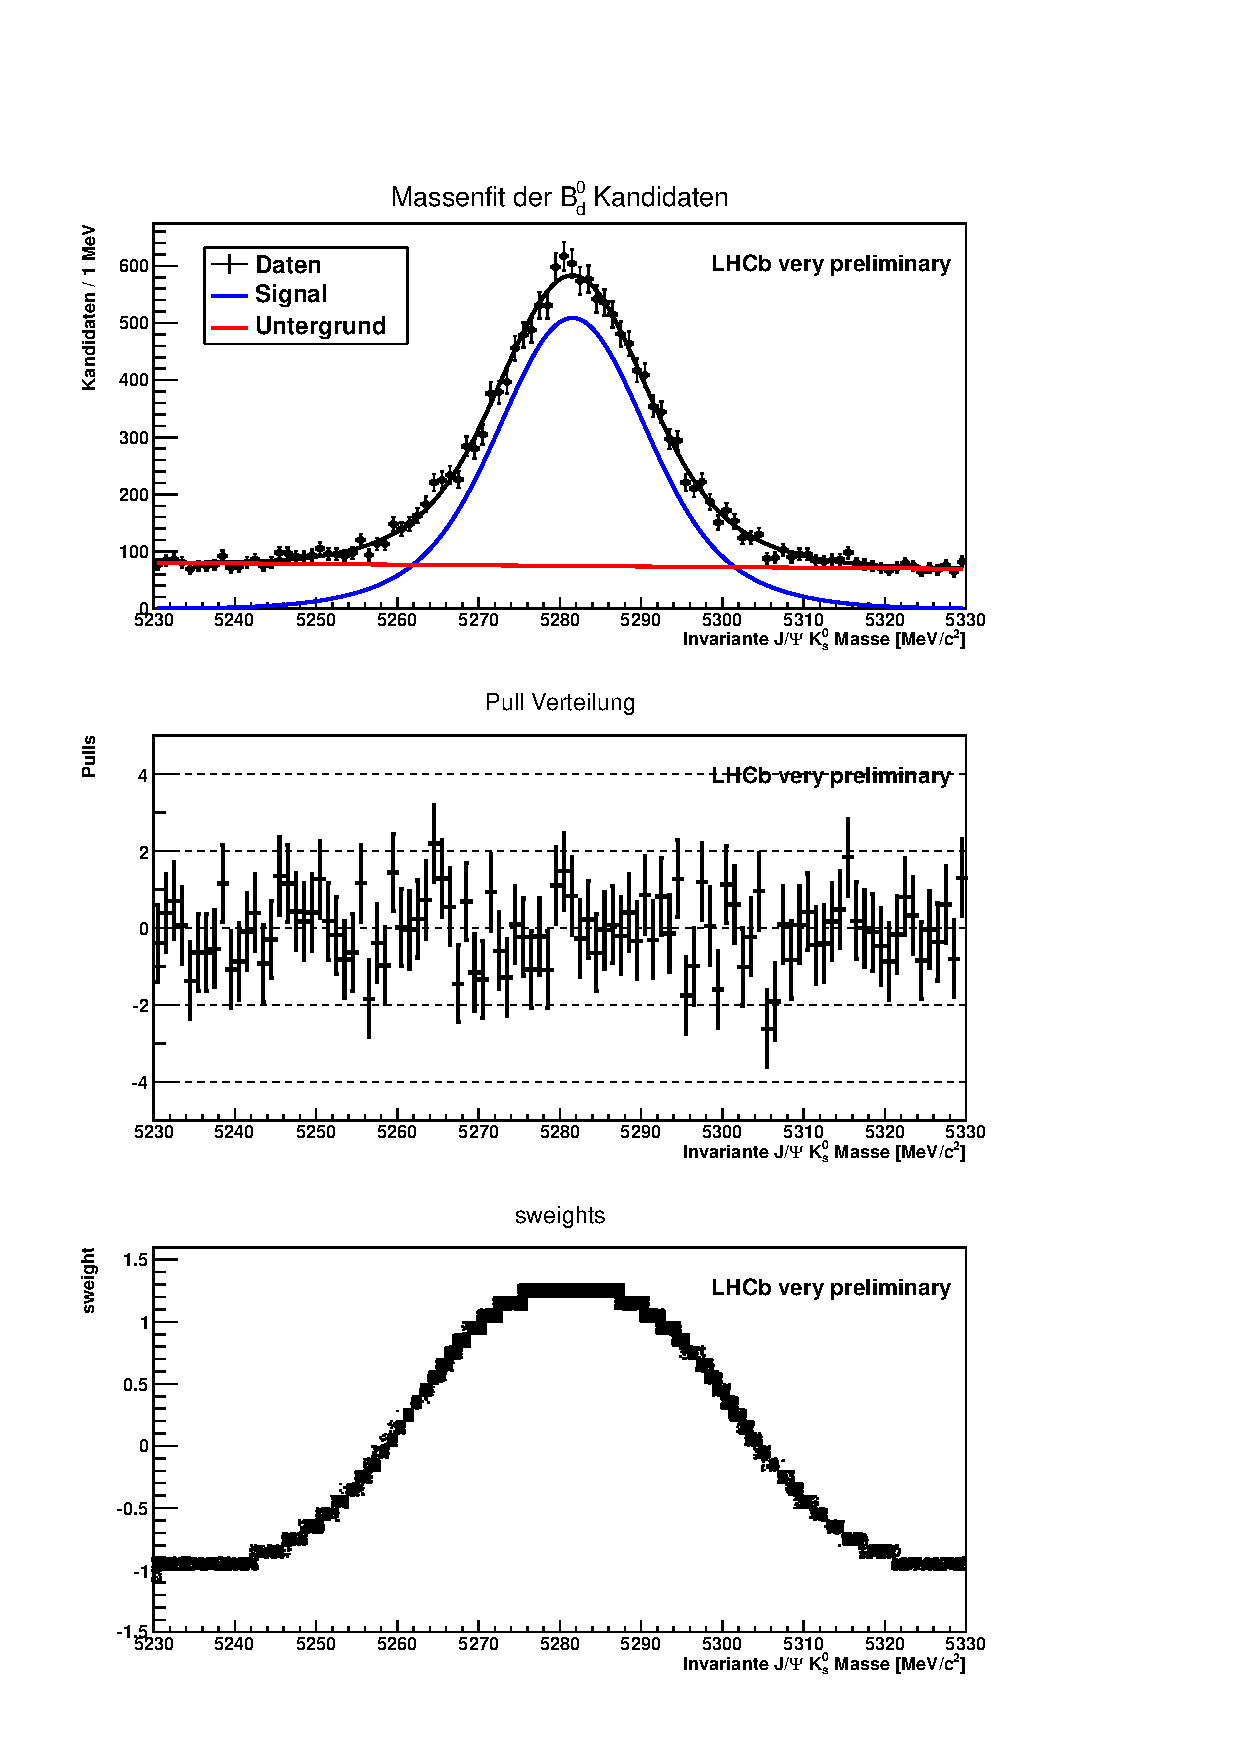
\includegraphics[width=\textwidth]{mass_fit}
\caption{Ergebnis des Massenfits}
\label{fig:fit_masse}
\end{figure}


\section{Fit der Eigenzeitverteilung} \label{kap:eigenzeitverteilung}
In diesem Abschnitt soll nun die Wahrscheinlichkeitsdichtefunktion der \Bd-Ei\-gen\-zeit\-ver\-tei\-lung entwickelt werden, die letztendlich zur Bestimmung der Asymmetrie-Amplitude $\SJPsi$ verwendet wird. Aus den Gleichungen \ref{eq:bd} und \ref{eq:bdbar} geht für $|\lambda_f|=1$ die theoretische Eigenzeitverteilung für ein \Bd\ bzw. \Bdbar\ hervor:
\begin{align}
\mathcal{P}_{\text{wahr}}(t, d_{\text{wahr}}) = \frac{1}{\mathcal{N}_t}\e^{-t/\tau}\left[1-d_{\text{wahr}}\SJPsi\sin(\sinarg)\right].
\end{align}
Durch die Einführung des Variablen $d_{\text{wahr}}$ wurden beide Verteilungen zu einer zusammengefasst. Dieses steht für den (wahren) Flavour des Mesons zum Zeitpunkt $t=0$. Ein anfängliches \Bd\ wird dabei durch $d_{\text{wahr}}=1$ beschrieben, ein \Bdbar\ durch $d_{\text{wahr}}=-1$. Die Normierung ist so gewählt, dass die Bedingung
\begin{align}
\sum_{d_{\text{wahr}}}\int_{t_{min}}^{t_{max}}\mathrm{d}t\mathcal{P}_{\text{wahr}}(t, d_{\text{wahr}}) = 1
\end{align}
erfüllt wird. Aufgrund zahlreicher detektorbedingten Effekte muss $\mathcal{P}_{\text{wahr}}(t, d_{\text{wahr}})$ modifiziert werden.

\subsection{Produktionsasymmetrie}
Der Detektor produziert \Bd- und \Bdbar-Mesonen nicht in exakt gleicher Zahl. Über die Produktionsraten $R_{\text{\Bdbar}}$ für ein \Bdbar\ bzw. $R_{\text{\Bd}}$ für ein \Bd\ ist die Produktionsasymmetrie definiert durch:
\begin{align}
\mu = A_P = \frac{R_{\text{\Bdbar}}-R_{\text{\Bd}}}{R_{\text{\Bdbar}}+R_{\text{\Bd}}}.
\end{align}
Anhand dieser Definition muss der Anteil an \Bd\ bzw. \Bdbar\ an der gesamten WDF gewichtet werden. Unter Verwendung des Kronecker-Deltas $\delta_{ij}$ lässt sich die WDF daher schreiben als:
\begin{align}
\nonumber \widetilde{\mathcal{P}}_{\text{wahr}}(t, d_{\text{wahr}}) &= \delta_{d_{\text{wahr}},1}(1-\mu)\mathcal{P}_{\text{wahr}}(t, 1) + \delta_{d_{\text{wahr}},-1}(1+\mu)\mathcal{P}_{\text{wahr}}(t, -1) \\
\nonumber &= (1-d_{\text{wahr}}\mu)\mathcal{P}_{\text{wahr}}(t, d_{\text{wahr}}) \\
&= \frac{1}{\mathcal{N}_t}\e^{-t/\tau}\left[1-d_{\text{wahr}}\mu - (d_{\text{wahr}}-\mu)\SJPsi\sin(\sinarg)\right].
\end{align}

Der Wert der Produktionsasymmetrie $\mu$ wurde in einigen Studien gemessen und wird der LHCb Analyse aus 2011 \cite{lhcb-paper} entnommen:
\begin{align}
\mu = -0,015 \pm 0,013 .
\end{align}

\subsection{Bestimmung des Anfangszustandes der \Bd-Mesonen (Flavour Tagging)} \label{kap:tagging}
Die Messung der indirekten \CP-Verletzung setzt voraus, dass der anfängliche Flavour des \Bd-Mesons bekannt ist. Den Vorgang zu entscheiden, ob ein rekonstruierter Signalkandidat ein $b$ oder $\overline{b}$ Quark enthält, nennt man \glqq Flavour Tagging\grqq. Hierzu werden sogenannte Tagging Algorithmen angewandt, die allerdings keine perfekten Ergebnisse lieferen. Von $N$ Kandidaten kann bei $N_U$ Kandidaten kein Anfangsflavour zugeordnet werden, bei $N_W$ ist er falsch und bei $N_R$ ist er richtig. Ein Maß für die Güte des Algorithmus ist die Tagging Effizienz
\begin{align}
\epsilon_{\text{tag}} = \frac{N_R+N_W}{N_R+N_W+N_U}
\end{align}
und die Fehlerwahrscheinlichkeit
\begin{align}
\omega = \frac{N_W}{N_R+N_W},
\end{align}
die die Wahrscheinlichkeit angibt, den Signalkandidaten den falschen Flavour zuzuordnen. Die Größe die es bei solchen Algorithmen zu maximieren gilt, ist die effektive Tagging Effizienz
\begin{align}
\epsilon_{\text{eff}} = \epsilon_{\text{tag}}(1-2\omega)^2 =: \epsilon_{\text{tag}} \mathcal{D}^2.
\end{align}

$\mathcal{D}$ wird auch Verwässerungsfaktor genannt. Bei dem in dieser Arbeit verwendeten Algorithmus handelt es sich um einen sog. Opposite Side Tagger (OST). Dieser nutzt aus, dass die meisten $b$ Quarks in Quark-Antiquark Paaren erzeugt werden. Dabei rekonstruiert der OST die Ladung der Zerfallsreste des entsprechenden Quark-Partners des \Bd-Mesons. Der Algorithmus berechnet aus kinematischen und geometrischen Daten eine Fehlerwahrscheinlichkeit $\eta^{OS} \in [0;0,5]$ für seine Flavour-Zuweisung (oder auch Tagging Entscheidung genannt), die im folgenden mit $d^{OS}$ bezeichnet wird. \cite{lhcb-paper}

Die vorhergesagte Fehlerwahrscheinlichkeit $\eta^{OS}$ muss allerdings noch auf diversen Zerfallskanälen kalibriert werden. Dies ist allerdings nicht Bestandteil dieser Arbeit, sondern wurde \cite{tagging} entnommen. Die Kalibrationsfunktion lautet:
\begin{align}
\omega(\eta^{OS}) = p_1\left(\eta^{OS}-\left\langle \eta^{OS} \right\rangle\right) + p_0 .
\end{align}
$\left\langle \eta^{OS} \right\rangle$ steht dabei für das arithmetische Mittel der $\eta^{OS}$-Verteilung. Aus \cite{tagging} erhält man
\begin{align}
p_0 &= 0,382 \pm 0,003 \\
p_1 &= 0,981 \pm 0,024 \\
\left\langle \eta^{OS} \right\rangle &= 0,382
\end{align}

Die im Algorithmus verwendeten geladenen Teilchen wie zum Beispiel ein $K^{\pm}$ können je nach Ladung zum Teil sehr unterschiedlich mit dem Detektormaterial reagieren. Daher kommt es auch zu unterschiedlichen Rekonstruktionseffizienzen für \Bd und \Bdbar. Entsprechend müssen zwei Kalibrationsfunktionen 
\begin{align}
\omega^{\text{\Bd}}(\eta^{OS}) &= p_1(\text{\Bd})\left(\eta^{OS}-\left\langle \eta^{OS} \right\rangle\right) + p_0(\text{\Bd}) , \\
\omega^{\text{\Bdbar}}(\eta^{OS}) &= p_1(\text{\Bdbar})\left(\eta^{OS}-\left\langle \eta^{OS} \right\rangle\right) + p_0(\text{\Bdbar})
\end{align}
berücksichtigt werden. Für die Differenzen der Kalibrationsparameter liefert \cite{tagging}
\begin{align}
\Delta p_0 &= p_0(\text{\Bd}) - p_0(\text{\Bdbar}) = 0,0045 \pm 0,0053 \\
\Delta p_1 &= p_1(\text{\Bd}) - p_1(\text{\Bdbar}) = 0,001 \pm 0,05 .
\end{align}
Während $p_1$ für \Bd und \Bdbar sehr gut übereinstimmen, muss man das bei $p_0$ differenzierter betrachten. Auch hier ist man zwar im $1\sigma$-Bereich kompatibel, anderen Studien der LHCb-Gruppe zeigen jedoch, dass die Tagging Asymmetrie $\Delta p_0$ berücksichtigt werden sollte, was auch hier geschieht. Dazu werden $\omega$ und $\Delta p_0$ so umdefiniert, dass
\begin{align}
\Delta p_0 &= \omega^{\text{\Bd}} - \omega^{\text{\Bdbar}}, \\
\omega^{\text{\Bd}} &= \omega + \frac{\Delta p_0}{2},  \\
\omega^{\text{\Bdbar}} &= \omega - \frac{\Delta p_0}{2}
\end{align}
gilt. Aufgrund der Fehlerwahrscheinlichkeit beim Tagging weicht die gemessene Eigenzeitverteilung von der tatsächlichen deutlich ab. Bei einem gemessenen \Bd\ ($d^{OS}=1$) handelt es sich in $(1-\omega^{\text{\Bd}})\%$ der Fälle auch tatsächlich um ein \Bd\ ($d_{wahr}=1$), in $\omega^{\text{\Bdbar}}\%$ der Fälle jedoch um ein wahres \Bdbar\ ($d_{wahr}=-1$). Damit nimmt die Wahrscheinlichkeitsdichtefunktion der gemessenen Verteilung die Form
\begin{alignat}{3}
\nonumber\widetilde{\mathcal{P}}_{\text{gem.}}(t, d^{OS}, \omega) &= && &&\delta_{d^{OS},1} \left[(1-\omega^{\text{\Bd}})\widetilde{\mathcal{P}}_{\text{wahr}}(t, d_{\text{wahr}}=1) + \omega^{\text{\Bdbar}}\widetilde{\mathcal{P}}_{\text{wahr}}(t, d_{\text{wahr}}=-1)\right]\\
\nonumber & && + &&\delta_{d^{OS},-1} \left[(1-\omega^{\text{\Bdbar}})\widetilde{\mathcal{P}}_{\text{wahr}}(t, d_{\text{wahr}}=-1) + \omega^{\text{\Bd}}\widetilde{\mathcal{P}}_{\text{wahr}}(t, d_{\text{wahr}}=1)\right] \\
\nonumber &= && &&\frac{1}{\mathcal{N}_t}\e^{-t/\tau} \left\lbrace 1-d\mu(1-2\omega)-d\Delta p_0 \right. \\
& && - && \left.\left[d(1-2\omega)-\mu(1-d\Delta p_0)\right]\SJPsi\sin(\sinarg)\right\rbrace \label{eq:fit_pdf_vorlaeufig}
\end{alignat}
In der letzten Zeile wurde für eine übersichtlichere Schreibweise $d:=d^{OS}$ verwendet.

\subsubsection{Effektive Tagging Effizienz}
Zum Ende dieses Abschnittes soll nun noch die effektive Tagging Effizienz bestimmt werden. Dazu wird zunächst die Tagging Effizienz berechnet. Es wird jeweils ein Massenfit nach Kapitel \ref{kap:massenfit} mit allen Kandidaten und nur mit Kandidaten, denen ein Flavour zugeordnet werden konnte durchgeführt. Aus beiden Fits wird der Anteil des Signals bestimmt und man erhält:
\begin{align}
\epsilon_{\text{tag}} = (29,43\pm 0,85)\%.
\end{align}
Es bleibt die Bestimmung von $\mathcal{D}:=1-2\omega$. Dazu wird zunächst die $\eta^{\text{OS}}$-Verteilung der Daten auf $\omega$ umkalibriert. Im Anschluss wird das gewichtete Mittel von $1-2\omega$ berechnet. Als Gewichte dienen zur Extrahierung des Signals die sWeights, die man aus dem zuvor durchgeführten Massenfit berechnet. Dies führt zu:
\begin{align}
\mathcal{D} = 0,2474\pm 0,0095.
\end{align}
Die Fehlerrechnung für $\mathcal{D}$ wird in \cite{2010-analyse} beschrieben. Aus beiden Werten folgt dann die effektive Tagging Effizienz von
\begin{align}
\epsilon_{\text{eff}} = \epsilon_{\text{tag}} \mathcal{D}^2 = (1,80\pm 0,15)\%
\end{align}

\subsection{Eigenzeitauflösung und -akzeptanz}
Der letzte Effekt, der noch berücksichtigt werden muss, ist die endliche, Ei\-gen\-zeit\-auf\-lösung des Detektors. Dies wird dadurch deutlich, dass es auch Ereignisse mit negativer Eigenzeit gibt. Da diese unphysikalisch sind und u.a. auf Auflösungseffekte zurückzuführen sind, werden genau diese Ereignisse zur Bestimmung einer Auflösungsfunktion verwendet. Es handelt sich dabei zwar nur um eine Näherung der Eigenzeitauflösung, wie aber später gezeigt wird, ist das nicht relevant für das Endergebnis von $\SJPsi$ (siehe Kap. \label{kap:aufloesung}). Wie in den Kapiteln \ref{kap:trigger} und \ref{kap:stripping} bereits erwähnt wurde, werden hierzu auf den Datensatz die High Level Trigger 2 Linie \texttt{Hlt2DiMuonJPsiDecision} sowie die Stripping Linie \texttt{BetaSBd2JPsiKsPrescaledLine} angewandt. Um die negativen Ereignisse zu sehen, darf natürlich keine Selektion auf die Lebensdauer erfolgen.

In dieser Arbeit wird das Modell der mittleren Eigenzeitauflösung verwendet. Als Akzeptanzfunktion wird ein dreifacher Gauß der Form
\begin{align}
\mathcal{R}(t) = \sum_{i=1}^{3} \frac{f_i}{\sqrt{2\pi}\sigma_i}\e^{-\frac{t^2}{2\sigma_i^2}}
\end{align}
mit dem gemeinsamen Mittelwert $0$, den unterschiedlichen Breiten $\sigma_i$, sowie den relativen Anteilen $f_i$ der einzelnen Gauß-Funktionen gewählt. Dabei ist $\sum f_i = 1$ zu beachten. Somit erübrigt sich, $f_3$ als eigenständigen Parameter zu betrachten, es wird $f_3 = 1 - f_1 - f_2$ verwendet. Um Signal von Untergrund zu trennen, wird ein sFit angewandt. Da der Zerfallsvertex der hier behandelten \Bd-Mesonen hauptsächlich durch den $\JPsi$-Vertex festgelegt wird, wird zur Bestimmung der sWeights die rekonstruierte $\JPsi$-Masse herangezogen (siehe \cite{6}). Entgegen dem Massenfit der \Bd-Mesonen aus Gleichung \ref{eq:pdf_masse} wird hier als Wahrscheinlichkeitsdichtefunktion die Summe aus einer Gauß- und einer CrystalBall-Funktion verwendet. Die Crystallball-Funktion hat eine gaußförmige Basis, aber einen zu kleineren Werten als dem Mittelwert hin asymmetrischen, abgeflachten Teil, der den Energieverlust durch Photonabstrahlung berücksichtigt. Sie ist durch
\begin{align}
\mathcal{CB}(m) = \frac{N}{\sigma\sqrt{2\pi}} \begin{cases} \exp(-\frac{(m-m_{\text{\Bd}})^2}{2\sigma^2}), & \text{für }\frac{m-m_{\text{\Bd}}}{\sigma}>-\alpha \\ \left(\frac{n}{|\alpha|}\right)^n \exp(-\frac{|\alpha|^2}{s}) \left(\frac{n}{|\alpha|}-|\alpha|-\frac{m-m_{\text{\Bd}}}{\sigma}\right)^{-n} & \text{für }\frac{m-m_{\text{\Bd}}}{\sigma}\leq -\alpha \end{cases} 
\end{align}
definiert. Der Parameter $\alpha$ beschreibt dabei den Übergang vom gaußartigen Teil in den auf einer Potenzfunktion besierenden abgeflachten Teil \cite{crystal_ball}. Abbildung \ref{fig:resolution} zeigt sowohl das Ergebnis des Massenfits als auch den Fit der Auflösungsfunktion. Die erhaltenen Parameter der Eigenzeitauflösung sind in Tabelle \ref{tab:resolution} aufgeführt.

\begin{figure}[hptb]
\centering
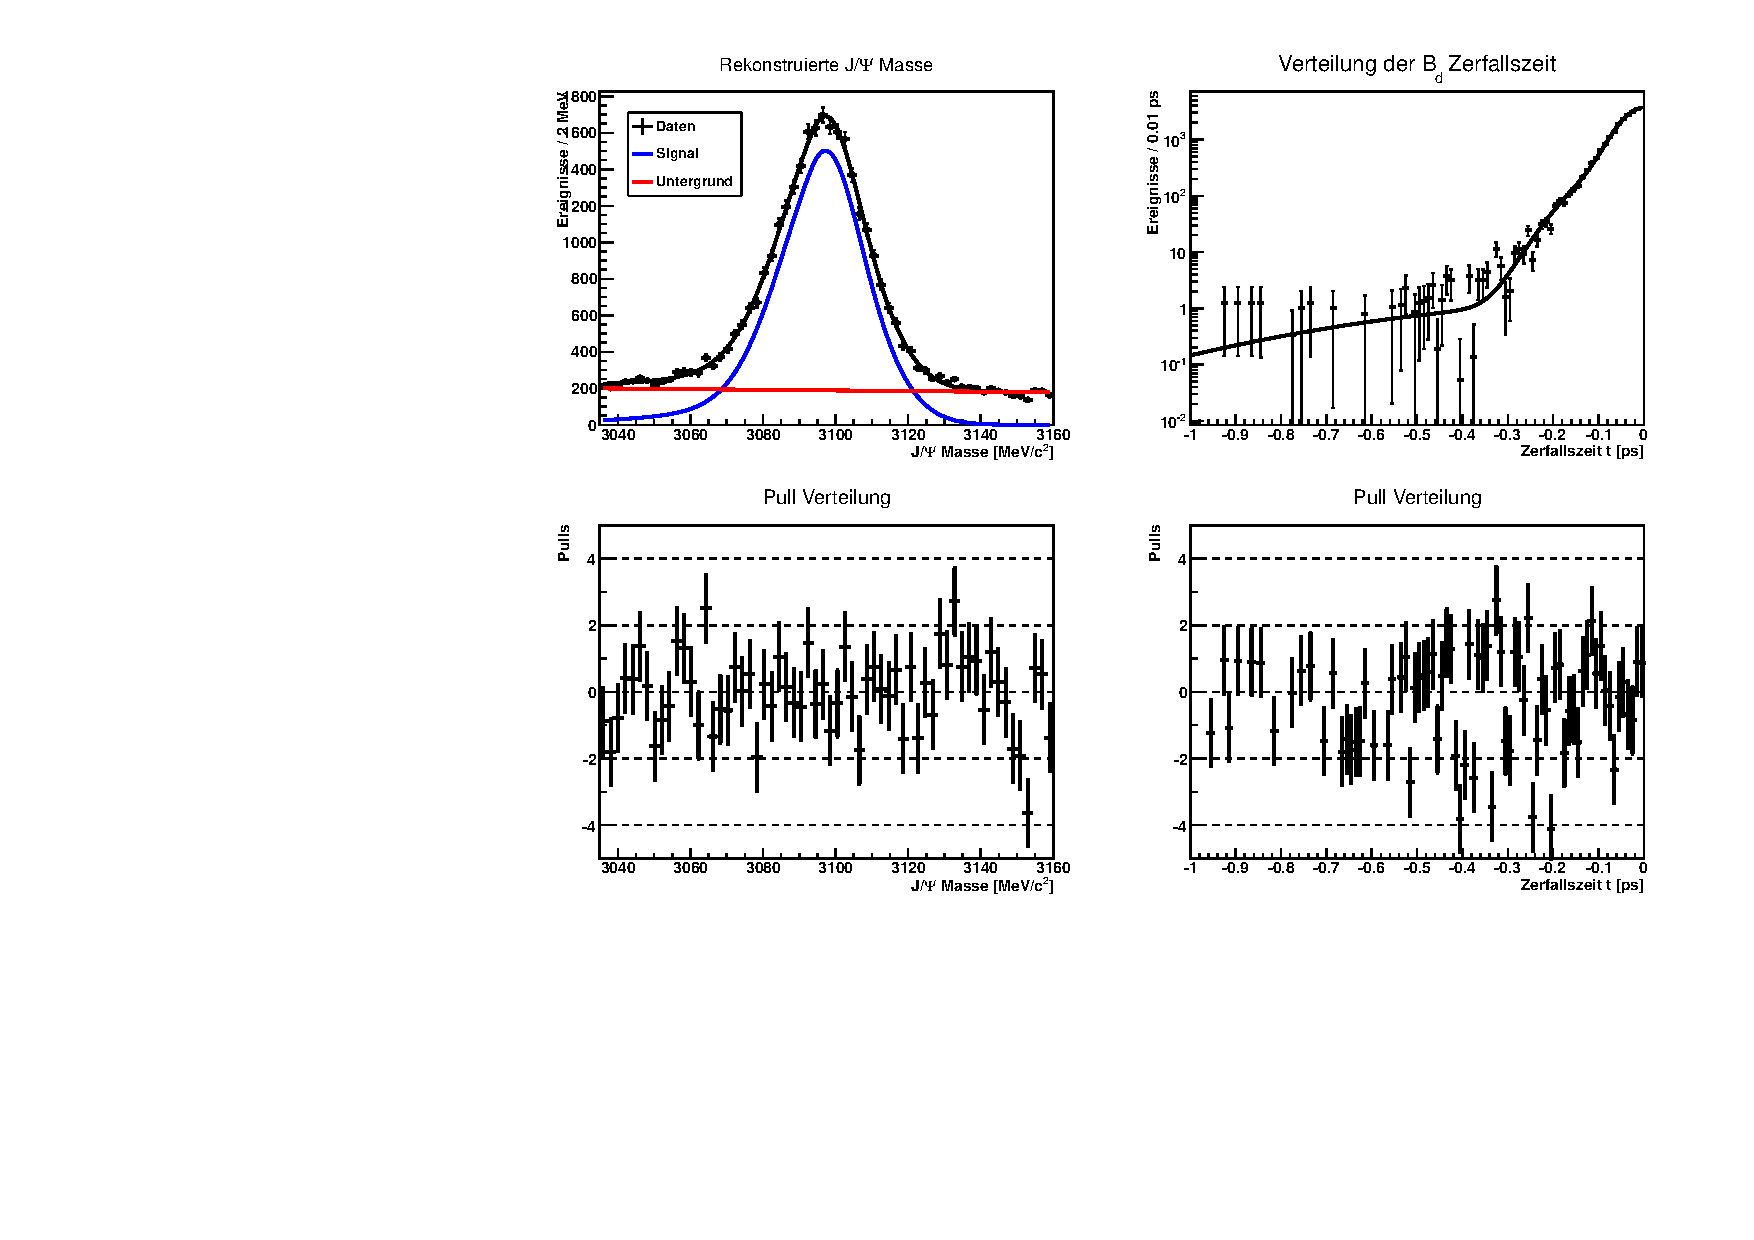
\includegraphics[width=\textwidth]{resolution}
\caption{Bestimmung der Auflösung: Die linke Hälfte zeigt den für die Bestimmung der sweights durchgeführten Fit an die rekonstruierte $\JPsi$-Masse (oben) und die dazugehörigen Pulls (unten), die rechte Hälfte den Fit der Auflösungsfunktion (oben) und die entsprechenden Pulls (unten)}
\label{fig:resolution}
\end{figure}

\begin{table}[hptb]
\centering
\caption{Ergebnisse des Fits der Eigenzeitauflösung}
\label{tab:resolution}
$\begin{array}{l r@{\pm}l l}
\hline 
\hline
\text{Parameter} & \multicolumn{2}{c}{\text{Wert}}&\\
\hline
\sigma_{1} & 0,480 & 0,070 & \ps\\
\sigma_{2} & 0,04396 & 0,00094 & \ps\\
\sigma_{3} & 0,0932 & 0,0034 & \ps\\
f_{1} & 0,00329 & 0,00099\\
f_{2} & 0,739 & 0,027\\ \hline
\sigma_{\text{eff}} & 0,0665 & 0,0013 \\ \hline \hline
\end{array}$   
\end{table}
Die effektive Auflösung beträgt
\begin{align}
\sigma_{\text{eff}} = \sum_{i=1}^3 = f_i \sigma_i^2 = (0,0665\pm 0,0013)\ps
\end{align}.
Im Fit wird die Auflösung dadurch berücksichtigt, dass die Wahrscheinlichkeitsdichtefunktion der Eigenzeitverteilung $\widetilde{\mathcal{P}}_{\text{gem.}}(t, \omega)$ (siehe Gleichung \ref{eq:fit_pdf_vorlaeufig}) mit der Auflösungsfunktion $\mathcal{R}(t)$ gefaltet werden muss. 

Ein weiterer Punkt, der berücksichtigt werden muss, ist die Eigenzeitakzeptanz des Detektors. Es werden hier keine großen Einflüsse erwartet, daher wird die Akzeptanzfunktion 
\begin{align}
\epsilon(t) = 1
\end{align}
gesetzt. Eine systematische Analyse und eine Abschätzung des Einflusses dieser Vernachlässigung findet sich in Kapitel \ref{kap:akzeptanz}.

\subsection{Fitfunktion}
Kombiniert man nun alle Effekte, die im vorigen Kapitel \ref{kap:eigenzeitverteilung}, aufgeführt und beschrieben wurden, so nimmt die Wahrscheinlichkeitsdichtefunktion für die Eigenzeitverteilung der \Bd-Mesonen die Form
\begin{alignat}{3}
\nonumber\mathcal{P}_{\text{gem.}}(t, d, \eta) &=\  &&  \epsilon(t)\left[\widetilde{\mathcal{P}}_{\text{gem.}}(t', d, \eta) \otimes \mathcal{R}(t-t')\right]\\
\nonumber &= &&\frac{1}{\mathcal{N}_t}\left[\e^{-t'/\tau} \left\lbrace 1-d\mu(1-2\omega)-d\Delta p_0 \right.\right.\\
& &&-\left.\vphantom{\frac{1}{\mathcal{N}_t}}\left.\left[d(1-2\omega)-\mu(1-d\Delta p_0)\right]\SJPsi\sin(\Delta m_d t')\right\rbrace\right]\otimes\mathcal{R}(t-t') \label{eq:fit_pdf}
\end{alignat}
an. Durch diesen Fit erhält man eine Abschätzung für den \CP-Parameter $\SJPsi$. In Gleichung \ref{eq:fit_pdf} bezeichnen $t'$ die wahre Eigenzeit, $t$ die rekonstruierte Eigenzeit, $\tau$ die \Bd-Lebensdauer, $\Delta m_d$ die Oszillationsfrequenz des \Bd-Mesons, $\mu$ die Produktionsasymmetrie sowie $d$ den durch die Flavour-Tagging Algorithmen bestimmten Anfangszustand des \Bd. Dabei gilt für \Bd-Mesonen $d=1$, für \Bdbar\ $d=-1$. Die Fehlerwahrscheinlichkeit des Flavour Taggings $\omega$ ist wiederum abhängig von der von den Algorithmen vorhergesagten Fehlerwahrscheinlichkeit $\eta$ gemäß
\begin{align}
\omega(\eta) = p_1\left(\eta-\left\langle\eta\right\rangle\right) + p_0.
\end{align}

Die \CP-Asymmetrie wird ebenfalls durch die Eigenzeitauflösung sowie fehlerhaftes Flavour Tagging beeinflusst, hier gilt für die Messung:
\begin{align}
\mathcal{A_{CP}}^{\text{meas}}(t) = (1-2\omega)\SJPsi \sin(\Delta m_d t') \otimes \mathcal{R}(t-t')
\end{align}


\section{Ergebnisse} \label{kap:fitergebnis}
Im Fit der Eigenzeitverteilung werden nicht alle Parameter laufen gelassen. Fixiert werden zum einen die Parameter der Eigenzeitauflösung (siehe Tab. \ref{tab:resolution}) und der Flavour-Tagging Kalibrationsparameter $\left\langle\eta\right\rangle = 0,382$. Des Weiteren werden einige Parameter eingeschränkt. Dies sind die Produktionasymmetrie $\mu$ sowie die Kalibrationsparameter $p_0$, $p_1$ und $\Delta p_0$. Die verwendeten Werte sind aus \cite{lhcb-paper} für $\mu$ beziehungsweise \cite{tagging} für $p_0$, $p_1$ und $\Delta p_0$ entnommen und in Tabelle \ref{tab:constrained_parameters} aufgeführt.

\begin{table}[hptb]
\centering
\caption{Parameter, die im Fit eingeschränkt werden.}
\label{tab:constrained_parameters}
$\begin{array}{l r@{\pm}l }
\hline 
\hline
\text{Parameter} & \multicolumn{2}{c}{\text{Wert}}\\
\hline
p_0 & 0,382 & 0,003 \\
p_1 & 0,981 & 0,024 \\
\Delta p_0 & 0,0045 & 0,0053 \\
\mu & -0,015 & 0,013 \\ \hline \hline
\end{array}$ 
\end{table}

Als Parameter, die frei laufen, bleiben dementsprechend die \CP-Asymmetrie Amplitude $\SJPsi$, die Lebensdauer $\tau$ sowie die Oszillationsfrequenz $\Delta m_d$ übrig. Während der gesamten Analyse wurde der Parameter $\SJPsi$ verdeckt (Fachjargon: \glqq geblindet\grqq). Dabei wird das eigentliche Ergebnis um einen dem Experimentator unbekannten Wert verschoben. Diese Verschiebung wird mittels einer Zeichenkette berechnet. Dies soll verhindern, dass sich der Experimentator an älteren Messungen oder dem Weltmittelwert etc. orientiert und dahingehend seine Analyse beeinflusst. Erst nach Beendigung aller systematischen Studien (siehe Kapitel \ref{kap:systematik}) und beim Verfassen dieser Arbeit wurde die wahre Abschätzung von $\SJPsi$ aufgedeckt. Diese sei hier schon einmal vorweggenommen:
\begin{align}
\SJPsi = xxx \pm 0,063     \label{eq:fit_result}
\end{align}

Alle Resultate des Fits sind in Tabelle \ref{tab:fit_results} aufgeführt. Die gemessene Eigenzeitverteilung sowie die dazugehörigen Fitkurven sind in Abbildung \ref{fig:fit_result} in Schwarz (für \Bd) und in Rot (\Bdbar) dargestellt.

\begin{table}[hptb]
\centering
\caption{Ergebnisse des Fits der Eigenzeitverteilung.}
\label{tab:fit_results}
$\begin{array}{l r@{\pm}l l}
\hline 
\hline
\text{Parameter} & \multicolumn{2}{c}{\text{Wert}}\\
\hline
\SJPsi & xxx & 0,063 &\\
\tau & (1,498 & 0,017) & \ps\\
\Delta m_d & (0,474 & 0,034) & \hbar\ps^{-1} \\ \hline
p_0 & 0,3815 & 0,0030 & \\
p_1 & 0,977 & 0,024 &\\
\Delta p_0 & 0,0049 & 0,0050 &\\
\mu & -0,020 & 0,013 &\\ \hline \hline
\end{array}$ 
\end{table}

\begin{figure}[hptb]
\centering
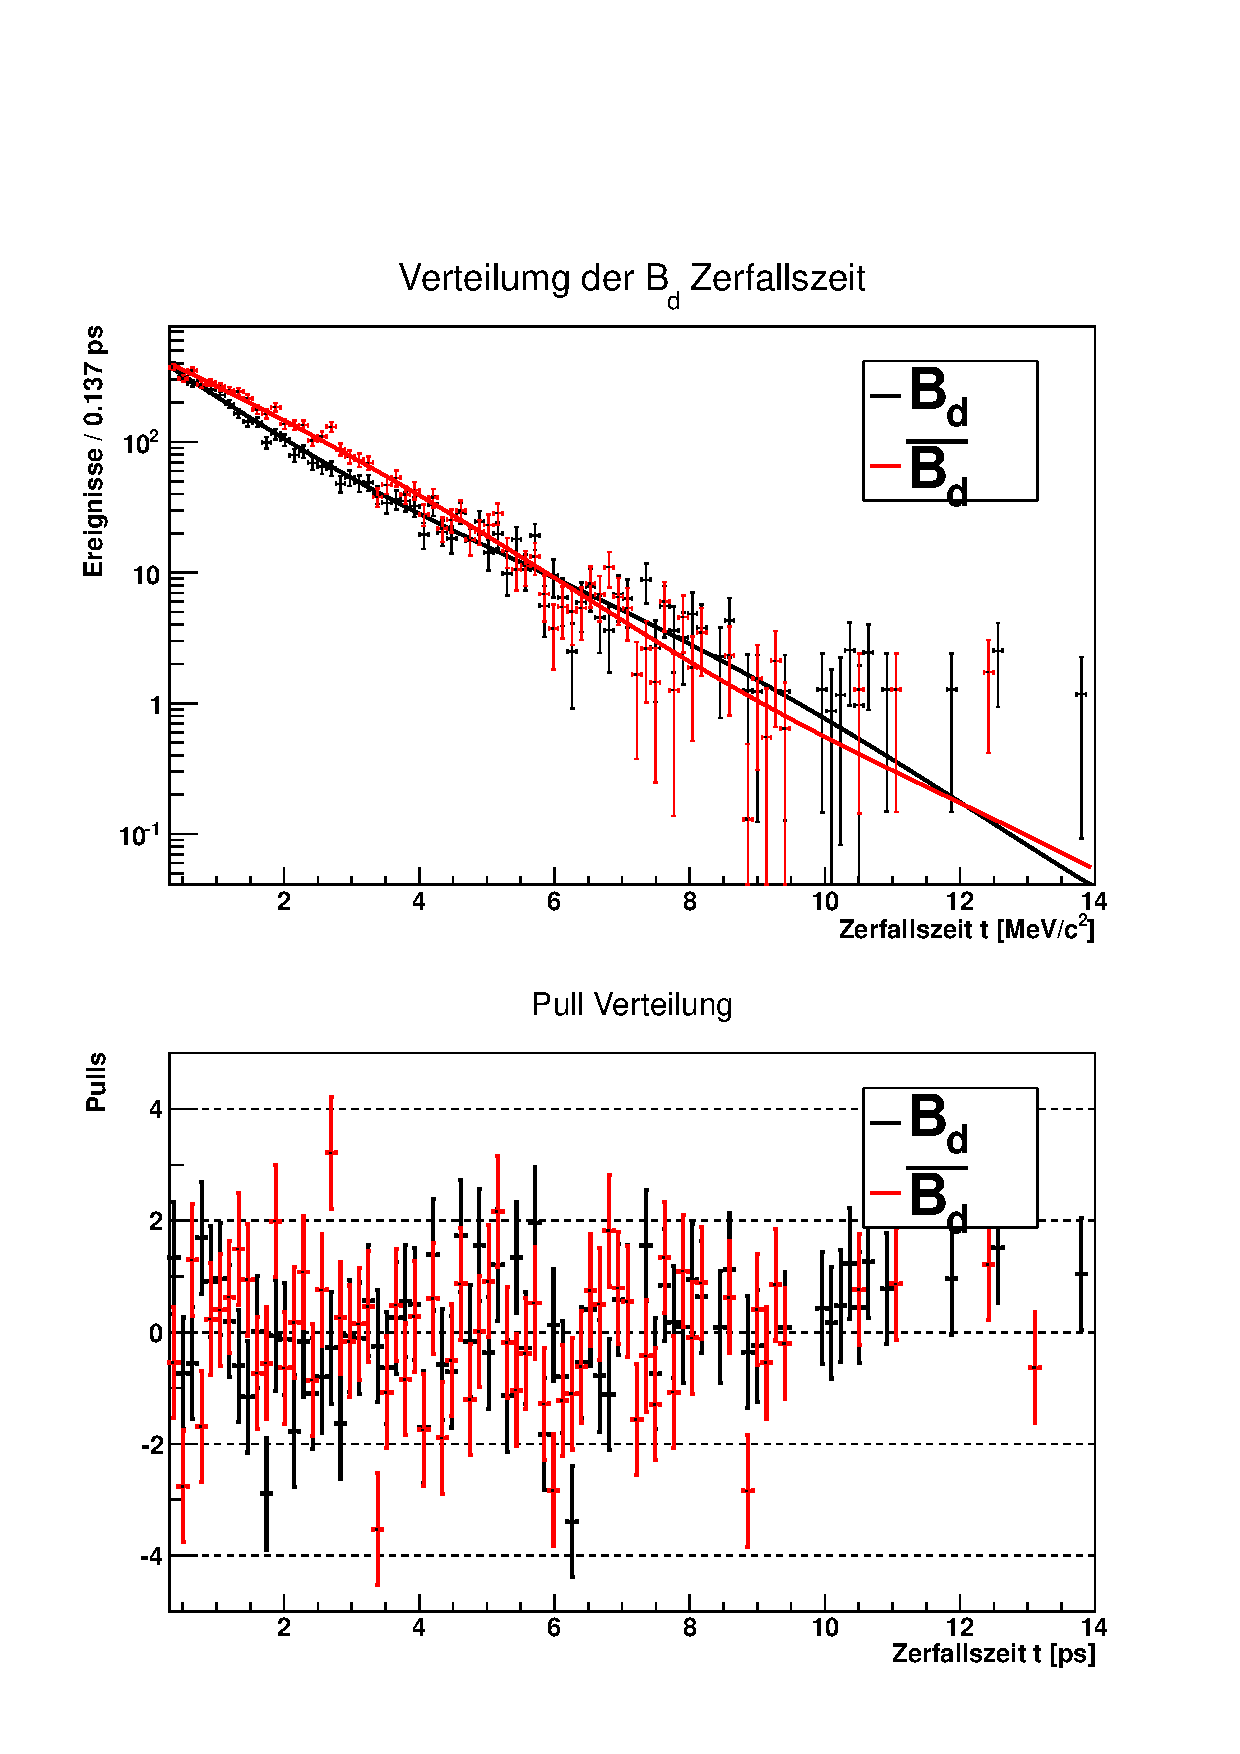
\includegraphics[width=\textwidth]{eigenzeitverteilung}
\caption{Ergebnis des Fits der Eigenzeitverteilung: Gemessene Eigenzeitverteilung der \Bd- (schwarz) bzw. \Bdbar-Mesonen (rot) mit entsprechendem Fitergebnis gemäß Gleichung \ref{eq:fit_pdf} und den Parametern aus Tabelle \ref{tab:fit_results} (oben) sowie dazugehörige Pull-Verteilung (unten).}
\label{fig:fit_result}
\end{figure}